\chapter{Introduction}
\label{ch:Introduction}

\section{General}

\subsection{Parkinson's Disease}

According to Patients Medical \cite{patients_medical_definition_2014}, \begin{quote}``Parkinson's disease is a progressive, neurodegenerative disease that occurs when the neurons within the brain responsible for producing the chemical dopamine become impaired or die. Dopamine is essential for the smooth control and coordination of the movement of voluntary muscle groups. Once approximately 80\% of the brain's dopamine producing cells no longer function, the symptoms of Parkinson's disease begin to appear. \dots Parkinson's disease may be termed as a progressive movement disorder that is distinguished by marked slow movements, tremors, and unstable posture.''\end{quote}

Especially in advanced stages of the Parkinson's disease (PD)\nomenclature{PD}{Parkinson's disease} many patients exhibit an episodic, brief inability to step that delays gait initiation or interrupts ongoing gait. This phenomenon is called freezing of gait and is often associated with an alternating shaking of the knees, termed as knee trembling. However, these clinical signs of balance or gait problems are not evident in early stages of the disease \cite{mancini_anticipatory_2009}\cite{jacobs_knee_2009}.

\subsection{Anticipatory Postural Adjustments}

To induce gait Anticipatory postural adjustments (APAs)\nomenclature{APAs}{Anticipatory Postural Adjustments} are made. The Encyclopedia of Neuroscience \cite[p.133]{woollacott_anticipatory_2009} defines APAs as "A predictive motor response that acts to counter, in a preemptive manner, the postural destabilization associated with a forthcoming movement." The centre of body mass (COM)\nomenclature{COM}{Centre of Mass} is accelerated forward and laterally over the stance foot to make sure that the body does not fall laterally toward the stepping foot during the swing phase \cite{woollacott_anticipatory_2009}. Figure \ref{fig:APAoverview} shows the whole process divided in three periods. Period S1 indicates the uncoupling of the centre of pressure (COP)\nomenclature{COP}{Centre of Pressure} and COM as the COP moves posteriorly and toward the intended stepping limb. Then, in the S2 period, the COP displaces mediolaterally toward the stance foot. Finally, during the S3 period the COP moves anteriorly under the stance foot \cite{hass_gait_2005-1}.

\begin{figure}
	\centering
	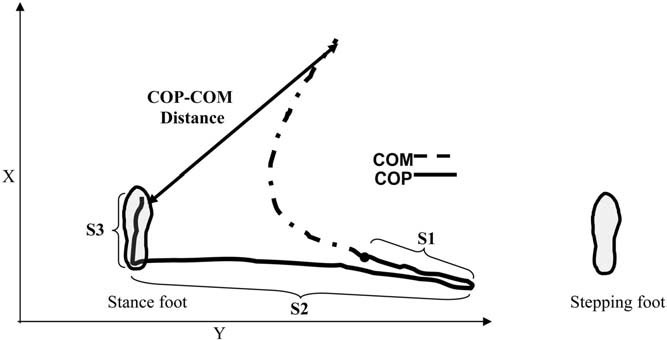
\epsfig{file=images/APA_overview, width=9cm}
	\caption{Anticipatory Postural Adjustments during forward-oriented gait initiation when stepping with the right foot. The arrow represents the distance between the COP-COM \cite{hass_gait_2005-1}}
	\label{fig:APAoverview}
\end{figure}


\section{Motivation}

Advanced PD can increasingly diminish quality of life, due to the fact that patients are dependent on help from others to accomplish daily tasks. Early diagnosis of PD could optimise early treatment. Currently new drugs are being developed and are expected to decelerate or stop the course of the disease in early stages \cite{botzel_motivation_2014}. Moreover an objective PD classification could evaluate longterm treatment success while testing these drugs.


\section{Goals}

The goal of the project is to carry out the so called Anticipatory Postural Analysis, which are the movements by a human subject between the moment he initiates gait and the first step. The medical community is interested in this procedure as it can be used for the diagnosis of neurodegenerative diseases such as Parkinson's. We aimed to build a classifier which is fed with data from both force plate and magnetic inertial measurement unit (MIMU)\nomenclature{MIMU}{Magnetic Intertial Measurement Unit} to distunguish between Parkinson patients and healthy subjects.


\section{State of the art}

There are several methods and devices to assess Parkinson's disease and to analyse Anticipatory Postural Adjustments. The state of the art at the beginning of the project is presented below.

\subsection{Rating scales}

One commonly used rating scale is the Unified Parkinson’s Disease Rating Scale (UPDRS)\nomenclature{UPDRS}{Unified Parkinson’s Disease Rating Scale} which is a short test performed by a physician \cite{klerk_long-term_2009}. The patient is rated on 31 different items (see table \ref{tab:UPDRS}) with a score of 0 (normal) to 4 (severely affected). Another method is the widely utilised and accepted Hoehn and Yahr scale (HY)\nomenclature{HY}{Hoehn and Yahr scale}. Parkinsonian motor impairment is categorised in 5 stages: Unilateral (Stage 1) to bilateral disease (Stage 2) without balance difficulties, to the presence of postural instability (Stage 3), loss of physical independence (Stage 4), up to being wheelchair- or bed-bound (Stage 5) \cite{goetz_movement_2004}. \citeauthor{klerk_long-term_2009} \cite{klerk_long-term_2009} mentioned the disadvantages such as subjectivity, short observation periods and unfamiliarity of the environment that both rating methods bring along.

\begin{table}[h]
\begin{tabular}{|l|l|l|}
\hline
Mentation, mood & Activities of daily & Motor examination \\
and behaivior & living & \\
\hline
\hline
Intellectual impairment & Speech & Speech \\

Thought disorder & Salivation & Facial expression\\

Depression & Swallowing & Tremor at rest \\

Motivation/initiative & Handwriting & Action or postural tremor of hands \\

& Use of eating utensils & Rigidity \\

& Dressing & Finger taps\\

& Hygiene & Hand movements\\

& Turning in bed & Rapid alternating movements of hands\\

& Falling & Food agility\\

& Freezing when walking & Arising from chair \\

& Walking & Posture\\

& Tremor & Gait\\

& Sensory Complaints & Posture stability\\

& & Body bradikinesia and hypokinesia \\
\hline
\end{tabular}
\label{tab:UPDRS}
\caption{UPDRS items adapted from \cite{herndon_handbook_2006}}
\end{table}

\subsection{Instrumentation}

In addition to the named subjective rating scales there are different devices used to quantify gait and posture and assess them ojectively. All of them come with certain pros and cons. The following devices have been used:

\begin{itemize}

\item Electromyographs: Electromyography is a technique for evaluating the electrical activity of skeletal muscels. Successive action potentials generated by muscle cells are measured by means of needle electrodes inserted into the muscle and displayed on a cathode-ray oscilloscope. Thus medical abnormalities can be detected. The instrument used to capture the visual recording, termed electromyogram, is called electromyograph. \cite{encyclopedia_britannica_electromyography_2014}.

\item Force plates: Force plates quantify the ground reaction force (GRF)\nomenclature{GRF}{Ground Reaction Force}, which is the force exerted to the human body by the ground. The GRF is a 3-dimensional vector with three orthogonal components. One component along the direction of gravity Fz one parallel to the ground in the sagittal plane and one parallel to the ground in the frontal plane voltage proportional to the force

\item Inertial sensors:

\item Camera based:

\end{itemize}

\subsection{Calibration}

Different calibration methods are used...


\subsection{Classification}

Different classification methods/techniques are used...

Signal processing

